\documentclass[11pt]{article}

\usepackage{latexsym}
\usepackage{amssymb}
\usepackage{amsthm}
\usepackage{enumerate}
\usepackage{amsmath}
\usepackage{cancel}
\usepackage{graphicx}
\numberwithin{equation}{section}

\setlength{\evensidemargin}{.25in}
\setlength{\oddsidemargin}{-.25in}
\setlength{\topmargin}{-.75in}
\setlength{\textwidth}{6.5in}
\setlength{\textheight}{9.5in}
\newcommand{\due}{November 28th, 2016}
\newcommand{\HWnum}{8}
\newcommand{\grad}{\bold\nabla}
\newcommand{\vecE}{\vec{E}}
\newcommand{\scrptR}{\vec{\mathfrak{R}}}
\newcommand{\kapa}{\frac{1}{4\pi\epsilon_0}}
\newcommand{\emf}{\mathcal{E}}
\newcommand{\unit}[1]{\ensuremath{\, \mathrm{#1}}}
\newcommand{\real}{\textnormal{Re}}
\newcommand{\Erf}{\textnormal{Erf}}
\newcommand{\sech}{\textnormal{sech}}
\newcommand{\scrO}{\mathcal{O}}
\newcommand{\levi}{\widetilde{\epsilon}}
\newcommand{\partiald}[2]{\ensuremath{\frac{\partial{#1}}{\partial{#2}}}}
\newcommand{\norm}[2]{\langle{#1}|{#2}\rangle}
\newcommand{\inprod}[2]{\langle{#1}|{#2}\rangle}
\newcommand{\ket}[1]{|{#1}\rangle}
\newcommand{\bra}[1]{\langle{#1}|}





\begin{document}
\begin{titlepage}
\setlength{\topmargin}{1.5in}
\begin{center}
\Huge{Physics 3320} \\
\LARGE{Principles of Electricity and Magnetism II} \\
\Large{Professor Ana Maria Rey} \\[1cm]

\huge{Homework \#\HWnum}\\[0.5cm]

\large{Joe Becker} \\
\large{SID: 810-07-1484} \\
\large{\due} 

\end{center}

\end{titlepage}



\section{Problem \#1}
\begin{enumerate}[(a)]
    \item
    For a waveguide whose cross-section is an equilateral triangle whose vertices are at
    $$(x,y) = \left\{(0,0),(a,a/\sqrt{3}),(a,-a/\sqrt{3})\right\}$$
    we can verify that the function
    $$\psi_{mn} = \sin\frac{l\pi{x}}{a}\sin\frac{(m-n)\pi{y}}{a\sqrt{3}} + \sin\frac{m\pi{x}}{a}\sin\frac{(n-l)\pi{y}}{a\sqrt{3}} + \sin\frac{n\pi{x}}{a}\sin\frac{(l-m)\pi{y}}{a\sqrt{3}}$$
    where $l\equiv-m-n$ satisfy the TM boundary conditions as shown in figure \ref{Triangle}
    \begin{figure}
        \centering
        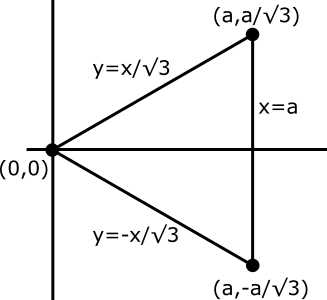
\includegraphics[width=0.5\textwidth]{Triangle.png}
        \caption{Equilateral triangle waveguide geometry.}
        \label{Triangle}
    \end{figure}
    If we recall the result from homework 7 we see that 
    $$\psi_{nm}(a,y) = \cancelto{0}{\sin{l\pi}}\sin\frac{(m-n)\pi{y}}{a\sqrt{3}}
        + \cancelto{0}{\sin{m\pi}}\sin\frac{(n-l)\pi{y}}{a\sqrt{3}}
        + \cancelto{0}{\sin{n\pi}}\sin\frac{(l-m)\pi{y}}{a\sqrt{3}} = 0$$
     and
    \begin{align*}
        \psi_{nm}(x,x/\sqrt{3}) &= \sin\frac{l\pi{x}}{a}\sin\frac{(m-n)\pi{x}}{3a}
            + \sin\frac{m\pi{x}}{a}\sin\frac{(n-l)\pi{x}}{3a}
            + \sin\frac{n\pi{x}}{a}\sin\frac{(l-m)\pi{x}}{3a}\\
        &= \frac{1}{2}\left[\cos\left(\frac{\pi{x}}{3a}(4m+2n)\right) - \cos\left(\frac{\pi{x}}{3a}(4m+2n)\right)\right.\\
        &\qquad+\cos\left(\frac{\pi{x}}{3a}(2m-2n)\right) - \cos\left(\frac{\pi{x}}{3a}(2m-2n)\right)\\
        &\qquad+\left.\cos\left(\frac{\pi{x}}{3a}(4n+2m)\right) - \cos\left(\frac{\pi{x}}{3a}(4n+2m)\right)\right]= 0
    \end{align*}
    Note that for the final boundary condition we can use the result from above and the fact
    that sine is a odd function to see
    \begin{align*}
        \psi_{nm}(x,-x/\sqrt{3}) &= \sin\frac{l\pi{x}}{a}\sin\frac{-(m-n)\pi{x}}{3a}
            + \sin\frac{m\pi{x}}{a}\sin\frac{-(n-l)\pi{x}}{3a}
            + \sin\frac{n\pi{x}}{a}\sin\frac{-(l-m)\pi{x}}{3a}\\
        &= -\left(\sin\frac{l\pi{x}}{a}\sin\frac{(m-n)\pi{x}}{3a}
            + \sin\frac{m\pi{x}}{a}\sin\frac{(n-l)\pi{x}}{3a}
            + \sin\frac{n\pi{x}}{a}\sin\frac{(l-m)\pi{x}}{3a}\right)\\
        &= -\psi_{nm}(x,x/\sqrt{3}) = 0
    \end{align*}
    So we see that all TM boundary conditions are met.

\item
    There exists a further set of TM modes, but not the modes described by the bisected 
    equilateral triangular waveguide described in part (a). Note that we already have met the
    boundary condition for the full equilateral triangle with an additional boundary 
    condition that $\psi_{mn}(x,0) = 0$. This implies that we should exchange the sine functions that depend on $y$
    to be cosine functions that depend on $y$, such that
    $$\psi_{mn} = \sin\frac{l\pi{x}}{a}\cos\frac{(m-n)\pi{y}}{a\sqrt{3}} + \sin\frac{m\pi{x}}{a}\cos\frac{(n-l)\pi{y}}{a\sqrt{3}} + \sin\frac{n\pi{x}}{a}\cos\frac{(l-m)\pi{y}}{a\sqrt{3}}$$
    Note that the boundary condition $\psi_{mn}(a,y) = 0$ still holds true as each sine function goes to zero. Next
    we check that
    \begin{align*}
        \psi_{mn}(x,x/\sqrt{3}) &= \sin\frac{l\pi{x}}{a}\cos\frac{(m-n)\pi{x}}{3a}
            + \sin\frac{m\pi{x}}{a}\cos\frac{(n-l)\pi{x}}{3a}
            + \sin\frac{n\pi{x}}{a}\cos\frac{(l-m)\pi{x}}{3a}\\
        &= \frac{1}{2}\left[\sin\left(\frac{\pi{x}}{3a}(3l-m+n)\right) + \sin\left(\frac{\pi{x}}{3a}(3l+m-n)\right)\right.\\
        &\qquad+\sin\left(\frac{\pi{x}}{3a}(3m-n+l)\right) + \sin\left(\frac{\pi{x}}{3a}(3m+n-l)\right)\\
        &\qquad+\left.\sin\left(\frac{\pi{x}}{3a}(3n-l+m)\right) + \sin\left(\frac{\pi{x}}{3a}(3n+l-m)\right)\right]\\
        &= \frac{1}{2}\left[\sin\left(\frac{\pi{x}}{3a}(-4m-2n)\right) + \sin\left(\frac{\pi{x}}{3a}(-2m-4n)\right)\right.\\
        &\qquad+\sin\left(\frac{\pi{x}}{3a}(2m-2n)\right) + \sin\left(\frac{\pi{x}}{3a}(4m+2n)\right)\\
        &\qquad+\left.\sin\left(\frac{\pi{x}}{3a}(4n+2m)\right) + \sin\left(\frac{\pi{x}}{3a}(2n-2m)\right)\right]\\
        &= \frac{1}{2}\left[\sin\left(\frac{\pi{x}}{3a}(4m+2n)\right) - \sin\left(\frac{\pi{x}}{3a}(4m+2n)\right)\right.\\
        &\qquad+\sin\left(\frac{\pi{x}}{3a}(2m-2n)\right) - \sin\left(\frac{\pi{x}}{3a}(2m-2n)\right)\\
        &\qquad+\left.\sin\left(\frac{\pi{x}}{3a}(4n+2m)\right) - \sin\left(\frac{\pi{x}}{3a}(4n+2m)\right)\right]\\
        &= 0
    \end{align*}
    Now for the final boundary condition we see that
    \begin{align*}
        \psi_{nm}(x,-x/\sqrt{3}) &= \sin\frac{l\pi{x}}{a}\cos\frac{-(m-n)\pi{x}}{3a}
            + \sin\frac{m\pi{x}}{a}\cos\frac{-(n-l)\pi{x}}{3a}
            + \sin\frac{n\pi{x}}{a}\cos\frac{-(l-m)\pi{x}}{3a}\\
        &= \left(\sin\frac{l\pi{x}}{a}\cos\frac{(m-n)\pi{x}}{3a}
            + \sin\frac{m\pi{x}}{a}\cos\frac{(n-l)\pi{x}}{3a}
            + \sin\frac{n\pi{x}}{a}\cos\frac{(l-m)\pi{x}}{3a}\right)\\
        &= \psi_{mn}(x,x/\sqrt{3}) = 0
    \end{align*}
    Note we can verify that this equation solves the \emph{Helmholtz Equation} by
    \begin{align*}
        \partiald{^2\psi}{x^2} + \partiald{^2\psi}{y^2} &= -\Omega^2\psi \\
                                                        &\Downarrow\\
        -\Omega^2\psi &= -\frac{\pi^2}{a^2}\left(\left(l^2+\frac{(m-n)^2}{3}\right)\sin\frac{l\pi{x}}{a}\cos\frac{(m-n)\pi{y}}{a\sqrt{3}}\right.\\
                      &\qquad+\left.\left(m^2+\frac{(n-l)^2}{3}\right)\sin\frac{m\pi{x}}{a}\cos\frac{(n-l)\pi{y}}{a\sqrt{3}}\right.\\
                      &\qquad+\left.\left(n^2+\frac{(l-m)^2}{3}\right)\sin\frac{n\pi{x}}{a}\cos\frac{(l-m)\pi{y}}{a\sqrt{3}}\right)\\
                      &= -\frac{4\pi^2}{3a^2}(m^2+n^2+mn)\psi_{mn}(x,y)
    \end{align*}
    Where we found that the eigenvalue is 
    $$\Omega^2_{mn} = \frac{4\pi^2}{3a^2}(m^2+n^2+mn)$$

\item
    To find the lowest frequency that can propagate through the equilateral triangular waveguide we note that we need
    to find the lowest mode that results in a oscillating field. This is when $m=1,n=1$ note that $m=0,n=0$ or $m=1,n=0$
    results in a null field.  We see that for these modes we have 
    $$\Omega = \frac{2\pi}{a} = \omega_{\textnormal{min}}$$
    Note that for the bisected triangular waveguide described in part (a) we have the lowest possible mode as 
    $m=2,n=1$ or $m=1,n=2$ due to the double sines. Note that the $m=1,n=1$ mode results in a null field,
    this implies that 
    $$\Omega^{\textnormal{bi}} = \sqrt{\frac{28}{3}}\frac{\pi}{a} = \omega^{\textnormal{bi}}_{\textnormal{min}}$$
\end{enumerate}

\pagebreak

\section{Problem \#2}
\begin{enumerate}[(a)]
\item
    Given the \emph{Lienard-Wiechert potentials}
    \begin{equation}
        \phi(\mathbf{r},t) = \frac{e}{R-\mathbf{v}\cdot\mathbf{R}} \qquad \mathbf{A}(\mathbf{r},t) = \frac{e\mathbf{v}}{R-\mathbf{v}\cdot\mathbf{R}}
    \end{equation}
    we can calculate the magnetic field which follows from an accelerating point charge by\
    \begin{align*}
        \mathbf{B} = \grad\times\mathbf{A} &= \grad\times\frac{e\mathbf{v}}{R-\mathbf{v}\cdot\mathbf{R}}\\
                              &= e\epsilon_{ijk}\partial_{j}\frac{v_k}{R-\mathbf{v}\cdot\mathbf{R}}\\
                              &= e\epsilon_{ijk}\frac{\partial_jv_k(R-\mathbf{v}\cdot\mathbf{R})-\partial_j(R-\mathbf{v}\cdot\mathbf{R})v_k}{(R-\mathbf{v}\cdot\mathbf{R})^2}
    \end{align*}
    Note the following results from the class notes
    \begin{align*}
        \partial_iR &= \frac{R_i}{R-\mathbf{v}\cdot\mathbf{R}}\\
        \partial_iR_j &= \delta_{ij} + \frac{v_jR_i}{R-\mathbf{v}\cdot\mathbf{R}}\\
        \partial_iv_j &= -\frac{\dot{v}_jR_i}{R-\mathbf{v}\cdot\mathbf{R}}
    \end{align*}
    we can calculate
    \begin{align*}
        \grad\times\mathbf{A} &= \frac{e\epsilon_{ijk}}{(R-\mathbf{v}\cdot\mathbf{R})^2}\left(-\frac{\dot{v}_kR_j\cancel{(R-\mathbf{v}\cdot\mathbf{R})}}{\cancel{R-\mathbf{v}\cdot\mathbf{R}}} - \frac{R_jv_k}{R-\mathbf{v}\cdot\mathbf{R}} + \partial_{j}(v_lR_l)v_k\right)\\
                              &= \frac{e\epsilon_{ijk}}{(R-\mathbf{v}\cdot\mathbf{R})^2}\left(-\dot{v}_kR_j - \frac{R_jv_k}{R-\mathbf{v}\cdot\mathbf{R}} + (\partial_{j}v_l)R_lv_k + (\partial_{j}R_l)v_lv_k\right)\\
                              &= \frac{e\epsilon_{ijk}}{(R-\mathbf{v}\cdot\mathbf{R})^2}\left(-\dot{v}_kR_j - \frac{R_jv_k}{R-\mathbf{v}\cdot\mathbf{R}} - R_lv_k\frac{\dot{v}_lR_j}{R-\mathbf{v}\cdot\mathbf{R}} + v_lv_k\delta_{jl} + v_lv_k\frac{v_lR_j}{R-\mathbf{v}\cdot\mathbf{R}}\right)\\
                              &= \frac{e}{(R-\mathbf{v}\cdot\mathbf{R})^3}\left(\mathbf{a}\times\mathbf{R}(R-\mathbf{v}\cdot\mathbf{R}) + \mathbf{v}\times\mathbf{R} + (\mathbf{a}\cdot\mathbf{R})(\mathbf{v}\times\mathbf{R})  - v^2(\mathbf{v}\times\mathbf{R})\right)\\
        &= \frac{e}{(R-\mathbf{v}\cdot\mathbf{R})^3}\left(\mathbf{a}\times\mathbf{R}(R-\mathbf{v}\cdot\mathbf{R}) + \mathbf{v}\times\mathbf{R}(1-v^2+\mathbf{a}\cdot\mathbf{R})\right)
    \end{align*}

\item
    Given that the electric field from a accelerating charge is given by
    \begin{equation}
        \mathbf{E} = \frac{e}{(R-\mathbf{v}\cdot\mathbf{R})^3}\left((1-v^2)(\mathbf{R}-\mathbf{v}R) + \frac{}{}\mathbf{R}\times\left[(\mathbf{R}-\mathbf{v}R)\times\mathbf{a}\right]\right)
    \end{equation}
    we can calculate the magnetic field by
    \begin{align*}
        \mathbf{B} &= \frac{\mathbf{R}\times\mathbf{E}}{R}\\
                   &= \frac{e}{R(R-\mathbf{v}\cdot\mathbf{R})^3}\left((1-v^2)\epsilon_{ijk}R_j(R_k-v_kR) + \epsilon_{ijk}R_j\epsilon_{klm}R_l\epsilon_{mno}(R_n-v_nR)a_o\right)\\
                   &= \frac{e}{R(R-\mathbf{v}\cdot\mathbf{R})^3}\left(-R(1-v^2)\epsilon_{ijk}R_jv_k + \epsilon_{ijk}R_j(\delta_{kn}\delta_{lo}-\delta_{ko}\delta_{ln})R_l(R_n-v_nR)a_o\right)\\
                   &= \frac{e}{R(R-\mathbf{v}\cdot\mathbf{R})^3}\left(-R(1-v^2)\epsilon_{ijk}R_jv_k + \epsilon_{ijk}R_j(R_la_l(R_k-v_kR) - R_l(R_l-v_lR)a_k)\right)\\
                   &= \frac{e}{R(R-\mathbf{v}\cdot\mathbf{R})^3}\left(R(1-v^2)\mathbf{v}\times\mathbf{R} + R(\mathbf{a}\cdot\mathbf{R})(\mathbf{v}\times\mathbf{R}) + (R^2-R\mathbf{v}\cdot\mathbf{R})\mathbf{a}\times\mathbf{R}\right)\\
                   &= \frac{e}{(R-\mathbf{v}\cdot\mathbf{R})^3}\left((R-\mathbf{v}\cdot\mathbf{R})\mathbf{a}\times\mathbf{R} + (1-v^2+\mathbf{a}\cdot\mathbf{R})\mathbf{v}\times\mathbf{R} \right)\\
    \end{align*}
    Recovering the result from part (a).
\end{enumerate}

\end{document}

